\documentclass[a4paper,12pt]{article}

\usepackage[utf8]{inputenc}
\usepackage[english]{babel}
\usepackage{hyperref}
\usepackage{fontenc}
\usepackage{graphicx}
\usepackage{makeidx}
\usepackage{color}
\usepackage{multirow}
\usepackage{tabularx}
\usepackage{longtable}
\usepackage{url}
\usepackage{titlesec}
\usepackage{listings}
\usepackage{xcolor}
\usepackage{colortbl}
\usepackage{geometry}
\usepackage{pdflscape}
\usepackage[toc,page,title]{appendix}

\geometry{
    a4paper,
    left=25mm,
    right=25mm,
    top=30mm,
    bottom=30mm,
 }

%%%%%%%%%%%%%%%%%%%%%%%%%%%%%
%%%%%%% CONFIGURATION %%%%%%%
%%%%%%%%%%%%%%%%%%%%%%%%%%%%%
%%%%%%%%%%%%%%%%%%%%%%%%%%%%%%%%%%%%%%
%%%%%%% SECTION CONFIGURATIONS %%%%%%%
%%%%%%%%%%%%%%%%%%%%%%%%%%%%%%%%%%%%%%
\newcommand{\sectionbreak}{\clearpage}

\setcounter{secnumdepth}{5}

\titleformat{\paragraph}
{\normalfont\normalsize\bfseries}{\theparagraph}{1em}{}
\titlespacing*{\paragraph}
{0pt}{3.25ex plus 1ex minus .2ex}{1.5ex plus .2ex}


%%%%%%%%%%%%%%%%%%%%%%%%%%%%%%%%%%%%%%
%%%%%%% LISTINGS CONFIGURATION %%%%%%%
%%%%%%%%%%%%%%%%%%%%%%%%%%%%%%%%%%%%%%
\definecolor{mybg}{rgb}{1,1,0.8}
\definecolor{mysoftblue}{rgb}{0.6,0.729,0.867}
\definecolor{mygreen}{rgb}{0,0.6,0}
\definecolor{mygray}{rgb}{0.5,0.5,0.5}
\definecolor{mymauve}{rgb}{0.58,0,0.82}

\lstset{ %
  backgroundcolor=\color{mysoftblue},    % choose the background color; you must add \usepackage{color} or \usepackage{xcolor}
  basicstyle=\ttfamily\scriptsize,        % the size of the fonts that are used for the code
  breakatwhitespace=false,         % sets if automatic breaks should only happen at whitespace
  breaklines=true,                 % sets automatic line breaking
  captionpos=b,                    % sets the caption-position to bottom
  commentstyle=\color{mygreen},    % comment style
  deletekeywords={...},            % if you want to delete keywords from the given language
  escapeinside={\%*}{*)},          % if you want to add LaTeX within your code (example: \%* int v; *) )
  extendedchars=true,              % lets you use non-ASCII characters; for 8-bits encodings only, does not work with UTF-8
  frame=single,                    % adds a frame around the code (none, single)
  keepspaces=true,                 % keeps spaces in text, useful for keeping indentation of code (possibly needs columns=flexible)
  keywordstyle=\color{blue},       % keyword style
  language=Java,                   % the language of the code
  otherkeywords={*,...},           % if you want to add more keywords to the set
  numbers=none,                    % where to put the line-numbers; possible values are (none, left, right)
  numbersep=5pt,                   % how far the line-numbers are from the code
  numberstyle=\tiny\color{mygray}, % the style that is used for the line-numbers
  rulecolor=\color{black},         % if not set, the frame-color may be changed on line-breaks within not-black text (e.g. comments (green here))
  showspaces=false,                % show spaces everywhere adding particular underscores; it overrides 'showstringspaces'
  showstringspaces=false,          % underline spaces within strings only
  showtabs=false,                  % show tabs within strings adding particular underscores
  stepnumber=2,                    % the step between two line-numbers. If it's 1, each line will be numbered
  stringstyle=\color{mymauve},     % string literal style
  tabsize=2,                       % sets default tabsize to 2 spaces
  title=\lstname,                  % show the filename of files included with \lstinputlisting; also try caption instead of title
  aboveskip=20pt,                  % space left avobe the listing
  belowskip=0pt,                   % space left below the listing
  columns=fullflexible             % to allow automatic copy from listings
}


%%%%%%%%%%%%%%%%%%%%%%%%%%%%%%%%%%%
%%%%%%% OTHER CONFIGURATION %%%%%%%
%%%%%%%%%%%%%%%%%%%%%%%%%%%%%%%%%%%

% Horizontal line
\newcommand{\HRule}{
  \rule{\linewidth}{0.5mm}
}

% Color box for comments
\newcommand{\colorComment}[1]{
\begin{table}[h]
    \centering
    \begin{tabular}{p{0.8\textwidth}}
        \cellcolor{orange}\begin{center}
	  #1 \\
        \end{center}
        \\
    \end{tabular}
\end{table}
}
\title{COMP Superscalar}
\author{Tracing Manual}
\def \compssversion {2.3.rc1809}

\makeindex

%%%%%%%%%%%%%%%%%%%%%%%%%%%%%
%%%%%%%% DOCUMENT %%%%%%%%%%%
%%%%%%%%%%%%%%%%%%%%%%%%%%%%%
\begin{document}

  %%%%%%%%%%%% TITLE PAGE %%%%%%%%%%%%%
  \hypersetup{pageanchor=false}
  \begin{titlepage} 
    \begin{center} 
      
\includegraphics[width=0.3\textwidth]{./Figures/Logos/degradado-naranja-compss.jpg}~\\[1cm] 
      \textsc{\LARGE COMP Superscalar}\\[1.5cm] 
      
      \HRule \\[0.4cm] 
      { \huge \bfseries COMPSs Tracing Manual \\[0.4cm] }
      \HRule \\[1.5cm] 

      { \large \textsc{Version: \compssversion}} \\[0.3cm]
      { \large \today } 
      
      \vfill 
      % Bottom of the page
      
\includegraphics[width=0.5\textwidth]{./Figures/bsc_280.jpg}~\\[1cm]
    \end{center} 
  \end{titlepage}
  \hypersetup{pageanchor=true}
  
  %%%%%%%% REFERENCE NOTES %%%%%%%%%%
  {
  
    This manual only provides information about the COMPSs tracing system. Specifically, it illustrates how to run COMPSs applications
    with tracing (using Extrae tool \footnote{For more information: \url{https://www.bsc.es/computer-sciences/extrae}}) and how to visualize, 
    interpret and analyze the obtained traces (using Paraver tool\footnote{For more information: \url{https://www.bsc.es/computer-sciences/performance-tools/paraver}]}).
    \newline

    For further information about the application execution, please refer to the \textit{COMPSs User Manual: Application execution
    guide} available at \url{http://compss.bsc.es/releases/compss/latest/docs/COMPSs_User_Manual_App_Exec.pdf}.
    \newline
    
    For further information about the application development, please refer to the \textit{COMPSs User Manual: Application development
    guide} available at \url{http://compss.bsc.es/releases/compss/latest/docs/COMPSs_User_Manual_App_Development.pdf}.

  }
  
  %%%%%%%% TABLE OF CONTENTS %%%%%%%%%%
  \pagenumbering{roman}
  \setcounter{tocdepth}{2}
  \tableofcontents
  \listoffigures
  \listoftables
    
  \newpage

  %%%%%%%%%%%%% CONTENTS %%%%%%%%%%%%%%
  \pagenumbering{arabic}
    
  \section{COMP Superscalar (COMPSs)}
\label{sec:Introduction}

COMP Superscalar (COMPSs) is a programming model which aims to ease the development of applications for distributed infrastructures, such as Clusters, Grids and Clouds. COMP superscalar also features a runtime system that exploits the inherent parallelism of applications at execution time.

For the sake of programming productivity, the COMPSs model has four key characteristics:

\begin{itemize}
 
 \item  {\bf Sequential programming:} COMPSs programmers do not need to deal with the typical duties of parallelization and distribution, such as thread creation and synchronization, data distribution, messaging or fault tolerance. Instead, the model is based on sequential programming, which makes it appealing to users that either lack parallel programming expertise or are looking for better programmability.
 
 \item  {\bf Infrastructure unaware:} COMPSs offers a model that abstracts the application from the underlying distributed infrastructure. Hence, COMPSs programs do not include any detail that could tie them to a particular platform, like deployment or resource management. This makes applications portable between infrastructures with diverse characteristics.
 
 \item  {\bf Standard programming languages:} COMPSs is based on the popular programming language Java, but also offers language bindings for Python and C/C++ applications. This facilitates the learning of the model, since programmers can reuse most of their previous knowledge.
 
 \item  {\bf No APIs:} In the case of COMPSs applications in Java, the model does not require to use any special API call, pragma or construct in the application; everything is pure standard Java syntax and libraries. With regard the Python and C/C++ bindings, a small set of API calls should be used on the COMPSs applications.

\end{itemize}


  
  \section{Trace Execution}
\label{sec:Execution}

COMPSs Runtime can generate a post-execution trace of the distributed execution of the application. This trace is useful for
performance analysis and diagnosis.

A trace file may contain different events to determine the COMPSs master state, the task execution state or the file-transfers.
Despite the fact that in the current release we do not support file-transfers, we intend to support them in a near future release.

During the execution of the application, an XML file is created at worker nodes to keep track of 
these events. At the end of the execution, all the XML files are merged to get a final trace file.

In the following sections we explain the command used for tracing, how the events are registered, 
in a process called instrumentation, how to visualize the trace file and make a good analysis of 
performance based on the data shown in the trace.

\subsection{Trace Command}
In order to obtain a post-execution trace file the option \textbf{-t}  must be added to the runcompss command. Next we provide an
example of the command execution with the tracing option enabled for the Hmmer java application.
\begin{lstlisting}[language=bash]
compss@bsc:~$ runcompss -t --classpath=/home/compss/workspace_java/hmmerobj/jar/hmmerobj.jar 
                        hmmerobj.HMMPfam 
                        /sharedDisk/Hmmer/smart.HMMs.bin /sharedDisk/Hmmer/256seq 
                        /home/compss/out.txt 2 8 -A 222
\end{lstlisting}
 

\subsection{Application Instrumentation}
The instrumentation is the process that intercepts different events of the application execution 
and keeps log of them. This will cause an overhead in the execution time of the application that 
the user should take into account, but the collected data will be extremely useful for performance 
analysis and diagnosis.

COMPSs Runtime uses the \textit{Extrae} tool to dynamically instrument the application and the \textit{Paraver} tool to visualize
the obtained tracefiles. Both tools are developped at \textit{BSC} and are available in its webpage \url{http://bsc.es} . 

At the worker nodes, in background, \textit{Extrae} keeps track of the events in an intermediate format 
file (with \textit{.mpit} extension). Inside the master node, at the end of the execution, \textit{Extrae} merges the 
intermediate files to get the final trace file, a \textit{Paraver} format file (.prv). See the visualization 
section \ref{sec:Visualization} in this manual for further information about the \textit{Paraver} tool.

When instrumenting the application \textit{Extrae} will output several messages. At the master node, \textit{Extrae} will show up its
initialization at the begining of the execution and the merging process and the paraver generation at the end of the execution. At the
worker nodes \textit{Extrae} will inform about the intermediate files generation every time a task is executed. Next we provide a 
summary of the \textit{stdout} generated by Hmmer java application execution with the trace flag enabled. 
\begin{lstlisting}[language=bash]
----------------- Executing hmmerobj.HMMPfam --------------------------

WARNING: IT Properties file is null. Setting default values
Welcome to Extrae 3.1.1rc (revision 3360 based on extrae/trunk)
Extrae: Warning! EXTRAE_HOME has not been defined!.
Extrae: Generating intermediate files for Paraver traces.
Extrae: Intermediate files will be stored in /home/compss/workspace_java/hmmerobj/jar
Extrae: Tracing buffer can hold 500000 events
Extrae: Tracing mode is set to: Detail.
Extrae: Successfully initiated with 1 tasks

Extrae: Warning! API tries to initialize more than once
Extrae:          Previous initialization was done by API

[   API]  -  Starting COMPSs Runtime v1.3 (build 20150821-1134.rnull)

...
...
...

[   API]  -  No more tasks for app 1
[   API]  -  Getting Result Files 1
[   API]  -  Execution Finished

Extrae: Intermediate raw trace file created : /home/compss/workspace_java/hmmerobj/jar/set-0/TRACE@bsc.0000031637000000000000.mpit
Extrae: Intermediate raw sym file created : /home/compss/workspace_java/hmmerobj/jar/set-0/TRACE@bsc.0000031637000000000000.sym
Extrae: Deallocating memory.
Extrae: Application has ended. Tracing has been terminated.

merger: Output trace format is: Paraver
merger: Extrae 3.1.1rc (revision 3360 based on extrae/trunk)

mpi2prv: Checking for target directory existance... exists, ok!
mpi2prv: Selected output trace format is Paraver
mpi2prv: Stored trace format is Paraver
mpi2prv: Parsing intermediate files
mpi2prv: Removing temporal files... done
mpi2prv: Congratulations! ./trace/hmmerobj.HMMPfam_compss_trace_1440151114.prv has been generated.

------------------------------------------------------------
\end{lstlisting}

For further information about \textit{Extrae} please visit the following site: 
\begin{center}
\url{http://www.bsc.es/computer-science/extrae} 
\end{center}
  
  \section{Visualization}
\label{sec:Visualization}

Paraver is the BSC tool for trace visualization. Trace events are encoded in Paraver format (.prv) by the Extrae tool. Paraver is a powerful
tool and allows users to show many views of the trace data using different configuration files. Users can manually load, edit or create
configuration files to obtain different tracing views. 

The following subsections explain how to load a trace file into Paraver, open the task events view using an already predefined 
configuration file, and how to adjust the view to display the data properly.

For further information about Paraver, please visit the following site:

\begin{center}
\url{http://www.bsc.es/computer-sciences/performance-tools/paraver}
\end{center}

\subsection{Trace Loading}
The final trace file in Paraver format (.prv) is at the base log folder of the application execution inside the trace folder. The fastest
way to open it is calling the Paraver binary directly using the tracefile name as the argument.

\begin{lstlisting}[language=bash]
wxparaver /path/to/trace/trace.prv
\end{lstlisting}
 
\subsection{Configurations}

To see the different events, counters and communications that the runtime generates, diverse configurations are available with the COMPSs
installation. To open one of them, go to the ``Load Configuration'' option in the main window and select ``File''. The configuration files
are under the following path for the default installation \verb|/opt/COMPSs/Dependencies/| \verb|paraver/cfgs/|. A detailed list of all the
available configurations can be found in Appendix \ref{sec:configs}.

The following guide uses the \textit{compss\_tasks.cfg} as an example to illustrate the basic usage of Paraver.
After accepting the load of the configuration file, another window appears showing the view. Figures \ref{fig:trace_1} and
\ref{fig:trace_2} show an example of this process.

\begin{figure}[ht!]
  \centering
    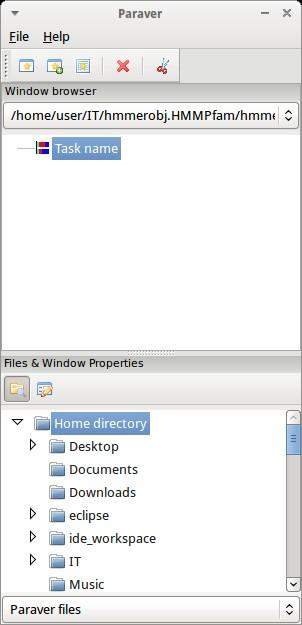
\includegraphics[width=0.45\textwidth]{./Sections/3_Visualization/Figures/1.jpeg}
    \caption{Paraver menu}
    \label{fig:trace_1}
\end{figure}

\begin{figure}[ht!]
  \centering
    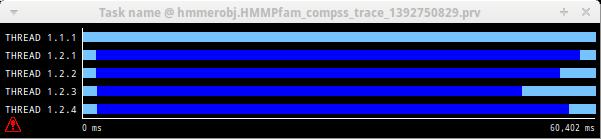
\includegraphics[width=1.0\textwidth]{./Sections/3_Visualization/Figures/2.jpeg}
    \caption{Trace file}
    \label{fig:trace_2}
\end{figure}

\subsection{View Adjustment}

In a Paraver view, a red exclamation sign may appear in the bottom-left corner (see Figure \ref{fig:trace_2} in the previous section). This
means that some event values are not being shown (because they are out of the current view scope), so little adjustments must be made to
view the trace correctly:

\begin{itemize}
 \item Fit window: modifies the view scope to fit and display all the events in the current window.
	\begin{itemize}
	    \item Right click on the trace window
	    \item Choose the option Fit Semantic Scale / Fit Both
	\end{itemize}
\end{itemize}

\begin{figure}[ht!]
  \centering
    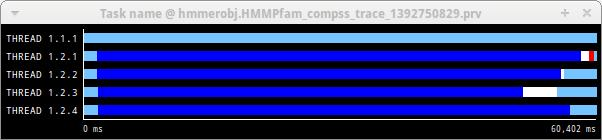
\includegraphics[width=1.0\textwidth]{./Sections/3_Visualization/Figures/3.jpeg}
    \caption{Paraver view adjustment: Fit window}
\end{figure}

\begin{itemize} 
 \item View Event Flags: marks with a green flag all the emitted the events.
	\begin{itemize}
	    \item Right click on the trace window
	    \item Chose the option View / Event Flags
	\end{itemize}
\end{itemize}
 
\begin{figure}[ht!]
  \centering
    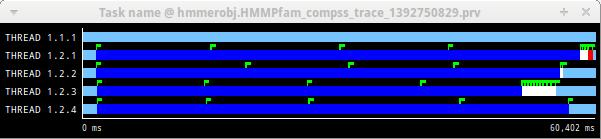
\includegraphics[width=1.0\textwidth]{./Sections/3_Visualization/Figures/4.jpeg}
    \caption{Paraver view adjustment: View Event Flags}
\end{figure}

\begin{itemize}
 \item Show Info Panel: display the information panel. In the tab ``Colors'' we can see the legend of the colors shown in the view.
	\begin{itemize}
	    \item Right click on the trace window
	    \item Check the Info Panel option
	    \item Select the Colors tab in the panel
	\end{itemize}
\end{itemize}

\begin{figure}[ht!]
  \centering
    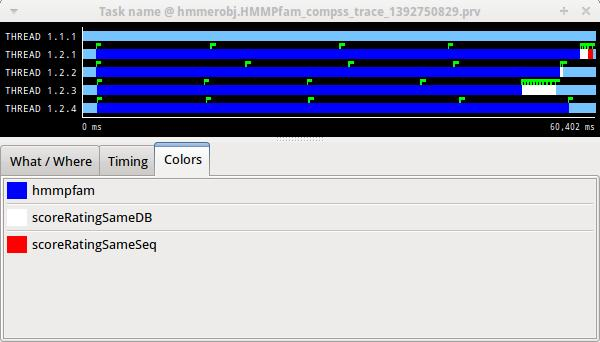
\includegraphics[width=1.0\textwidth]{./Sections/3_Visualization/Figures/5.jpeg}
    \caption{Paraver view adjustment: Show info panel}
\end{figure}

\begin{itemize}
 \item Zoom: explore the tracefile more in-depth by zooming into the most relevant sections.
	\begin{itemize}
	    \item Select a region in the trace window to see that region in detail
	    \item Repeat the previous step as many times as needed
	    \item The undo-zoom option is in the right click panel
	\end{itemize}
\end{itemize}

\begin{figure}[ht!]
  \centering
    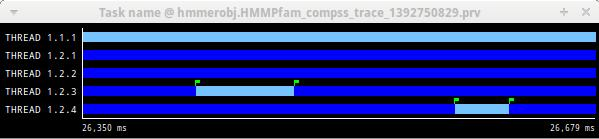
\includegraphics[width=1.0\textwidth]{./Sections/3_Visualization/Figures/6.jpeg}
    \caption{Paraver view adjustment: Zoom configuration}
\end{figure}

\begin{figure}[ht!]
  \centering
    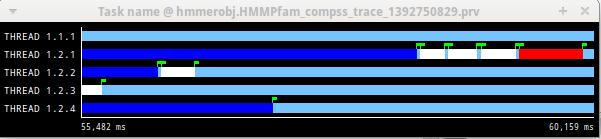
\includegraphics[width=1.0\textwidth]{./Sections/3_Visualization/Figures/6_2.jpeg}
    \caption{Paraver view adjustment: Zoom configuration}
\end{figure}

  
  \section{Interpretation}
\label{sec:Interpretation}

This section explains how to interpret a trace view once it has been adjusted as 
described in the previous section.

\begin{itemize}
 \item The trace view has on its horizontal axis the execution time and on the vertical 
       axis one line for the master at the top, and below it, one line for each of the workers.
 \item In a line, the light blue color is associated with an idle state, i.e. there is no event at that time.
 \item Whenever an event starts or ends a flag is shown.
 \item In the middle of an event, the line shows a different color. Colors are assigned depending on the event type.
 \item The info panel contains the legend of the assigned colors to each event type.
\end{itemize}

\begin{figure}[ht!]
  \centering
    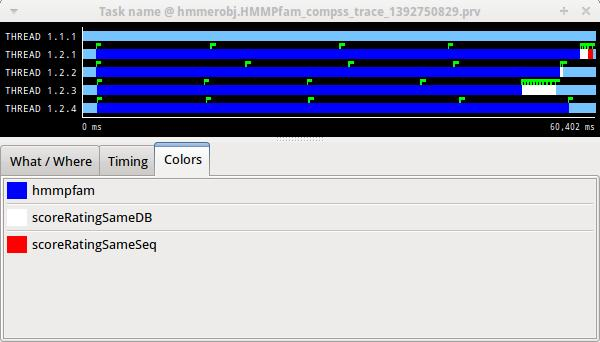
\includegraphics[width=\textwidth]{./Sections/4_Interpretation/Figures/7.jpeg}
    \caption{Trace interpretation}
\end{figure}

  \section{Analysis}
\label{sec:Analysis}
This section gives some tips to analyze a COMPSs trace from two different points of view:
graphically and numerically.

\subsection{Graphical Analysis}
The main concept is that computational events, the task events in this case, must be well 
distributed among all workers to have a good parallelism, and the duration of task events 
should be also balanced, this means, the duration of computational bursts.

\begin{figure}[ht!]
  \centering
    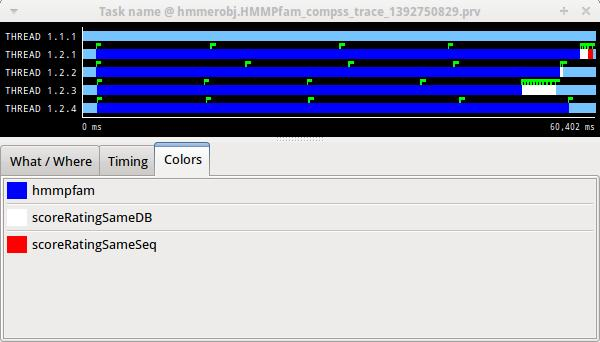
\includegraphics[width=1.0\textwidth]{./Sections/5_Analysis/Figures/8.jpeg}
    \caption{Basic trace view of a Hmmpfam execution.}
\end{figure}

In the previous trace view, all the tasks of type ``hmmpfam'' in dark blue appear to be well 
distributed among the four workers, each worker executes four ``hmmpfam'' tasks.

However, some workers finish earlier than the others, worker 1.2.3 finish the first and worker 1.2.1 
the last. So there is an imbalance in the duration of ``hmmpfam'' tasks. The programmer should 
analyze then whether all the tasks process the same amount of input data and do the same thing 
in order to find out the reason for such imbalance.

Another thing to highlight is that tasks of type ``scoreRatingSameDB'' are not equally distributed 
among all the workers. Some workers execute more tasks of this type than the others. 
To understand better what happens here, one needs to take a look to the execution graph and also zoom 
in the last part of the trace.

\begin{figure}[ht!]
  \centering
    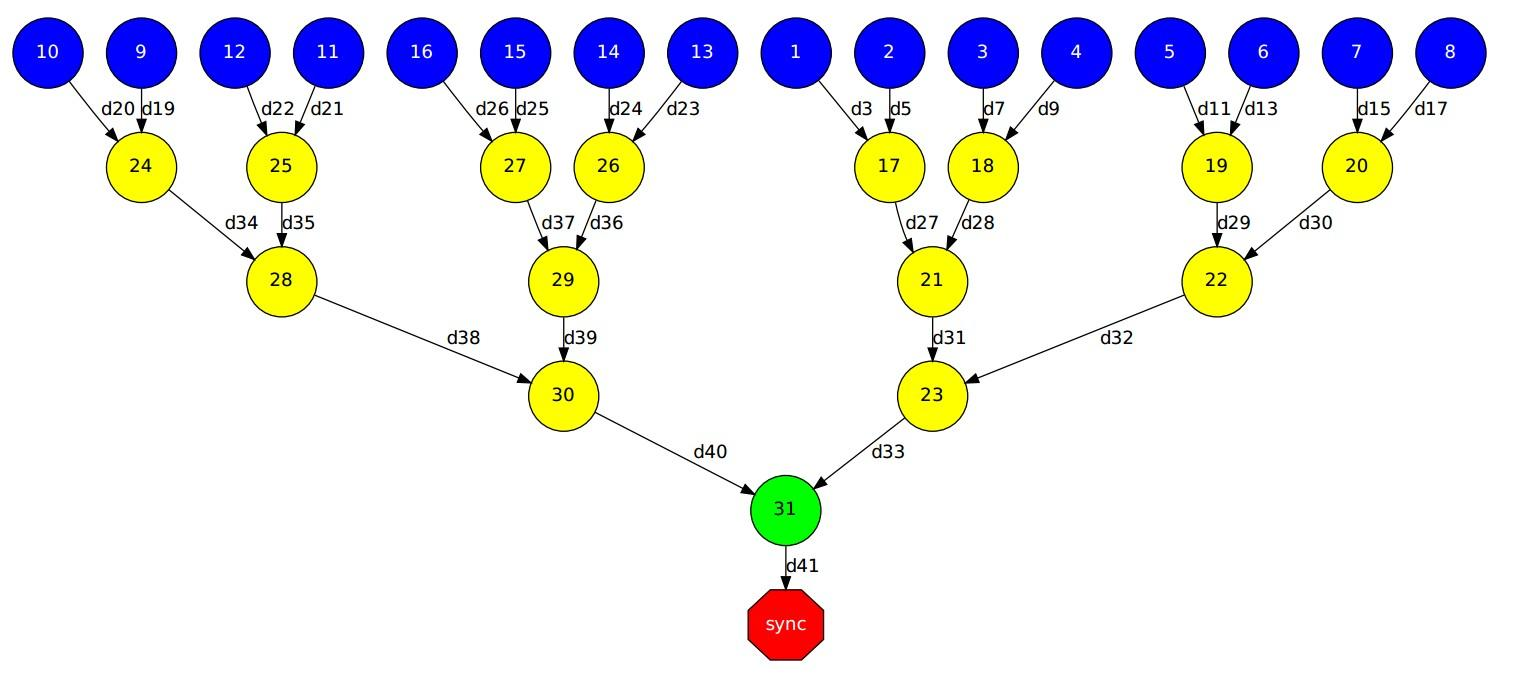
\includegraphics[width=1.0\textwidth]{./Sections/5_Analysis/Figures/9.jpeg}
    \caption{Data dependencies graph of a Hmmpfam execution.}
\end{figure}

\begin{figure}[ht!]
  \centering
    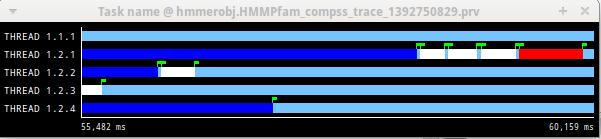
\includegraphics[width=1.0\textwidth]{./Sections/5_Analysis/Figures/10.jpeg}
    \caption{Zoomed in view of a Hmmpfam execution.}
\end{figure}

There is only one task of type ``scoreRatingSameSeq''. This task appears in red in the trace 
(and in light-green in the graph). With the help of the graph we see that the ``scoreRatingSameSeq'' 
task has dependences on tasks of type ``scoreRatingSameDB'', in white (or yellow).

When the last task of type ``hmmpfam'' (in dark blue) ends, the previous dependencies are solved, 
and if we look at the graph, this means going across a path of three dependencies of type 
``scoreRatingSameDB'' (in yellow). Moreover, because these are sequential dependencies (one depends 
on the previous) no more than a worker can be used at the same time to execute the tasks. 
This is the reason of why the last three task of type ``scoreRatingSameDB'' (in white) are 
executed in worker 1.2.1 sequentially.

\subsection{Numerical Analysis}
Here we show another trace from a different parallel execution of the Hmmer program.
 
\begin{figure}[ht!]
  \centering
    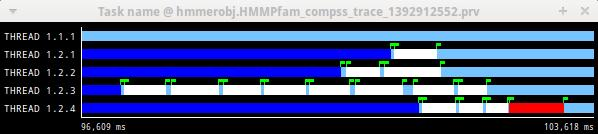
\includegraphics[width=1.0\textwidth]{./Sections/5_Analysis/Figures/11.jpeg}
    \caption{Original sample trace interval corresponding to the obtained Histogram.}
\end{figure} 
 
Paraver offers the possibility of having different histograms of the trace events. 
Click the ``New Histogram'' button in the main window and accept the 
default options in the ``New Histogram'' window that will appear.

\begin{figure}[ht!]
  \centering
    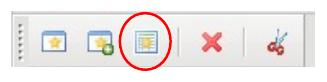
\includegraphics[width=0.5\textwidth]{./Sections/5_Analysis/Figures/12.jpeg}
    \caption{Paraver Menu - New Histogram}
\end{figure}

After that, the following table is shown. In this case for each worker, the time spent 
executing each type of task is shown. Task names appear in the same color than in the 
trace view. The color of a cell in a row corresponding to a worker ranges from 
light-green for lower values to dark-blue for higher ones. This conforms a color based histogram.

\begin{figure}[ht!]
  \centering
    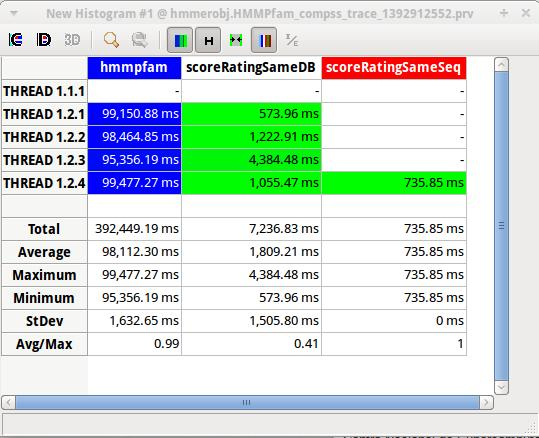
\includegraphics[width=0.8\textwidth]{./Sections/5_Analysis/Figures/13.jpeg}
    \caption{Hmmpfam histogram corresponding to previous trace}
\end{figure}
 
The previous table also gives, at the end of each column, some extra statistical 
information for each type of tasks (as the total, average, maximum or minimum values, etc.).

\newpage
In the window properties of the main window, it is possible to change the semantic of the statistics 
to see other factors rather than the time, for example, the number of bursts.

\begin{figure}[ht!]
  \centering
    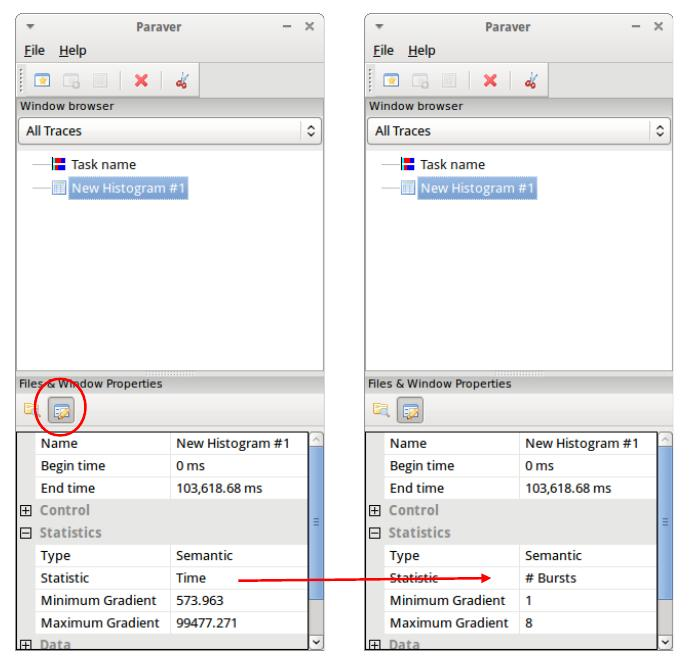
\includegraphics[width=0.8\textwidth]{./Sections/5_Analysis/Figures/14.jpeg}
    \caption{Paraver histogram options menu}
\end{figure}

\newpage
In the same way as before, the following table shows for each worker the number of bursts 
for each type of task, this is, the number or tasks executed of each type. Notice the gradient 
scale from light-green to dark-blue changes with the new values.

\begin{figure}[ht!]
  \centering
    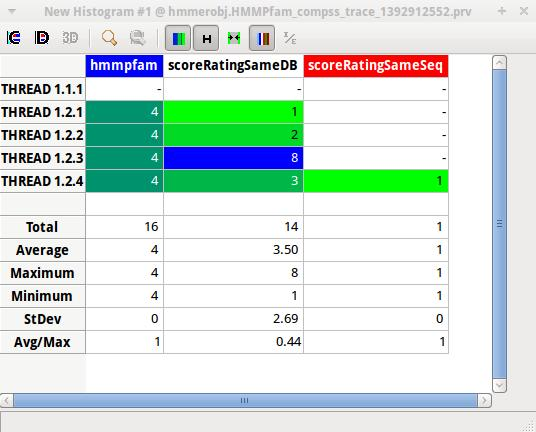
\includegraphics[width=0.8\textwidth]{./Sections/5_Analysis/Figures/15.jpeg}
    \caption{Hmmpfam histogram with the number of bursts}
\end{figure}
  
  \newpage

  \begin{appendices}
  
  \section{PAPI: Hardware Counters}
\label{sec:papi}

The applications instrumentation supports hardware counters through the performance API (PAPI). In order to use it, PAPI needs to be present on the machine before installing
COMPSs. 

During COMPSs installation it is possible to check if PAPI has been detected in the Extrae config report:

\begin{lstlisting}[language=bash]
Package configuration for Extrae 3.3.0 based on extrae/trunk rev. 3966:
-----------------------
Installation prefix: /opt/COMPSs/Dependencies/extrae
Cross compilation: no
...
...
...

Performance counters: yes
  Performance API: PAPI
  PAPI home: /usr
  Sampling support: yes
\end{lstlisting}


PAPI installation and requirements depend on the OS. On Ubuntu 14.04 it is available under textit{papi-tools} package; on OpenSuse textit{papi} and textit{papi-dev}.
For more information check \url{https://icl.cs.utk.edu/projects/papi/wiki/Installing_PAPI}.

Extrae only supports 8 active hardware counters at the same time. Both basic and advanced mode have the same default counters list:

\begin{description}
 \item [PAPI\_TOT\_INS] Instructions completed
 \item [PAPI\_TOT\_CYC] Total cycles
 \item [PAPI\_LD\_INS] Load instructions
 \item [PAPI\_SR\_INS] Store instructions
 \item [PAPI\_BR\_UCN] Unconditional branch instructions
 \item [PAPI\_BR\_CN] Conditional branch instructions
 \item [PAPI\_VEC\_SP] Single precision vector/SIMD instructions
 \item [RESOURCE\_STALLS] Cycles Allocation is stalled due to Resource Related reason
\end{description}

The XML config file contains a secondary set of counters. In order to activate it just change the \textit{starting-set-distribution} from 2 to 1 under the \textit{cpu} tag. The second set provides the following information:

\begin{description}
 \item [PAPI\_TOT\_INS] Instructions completed
 \item [PAPI\_TOT\_CYC] Total cycles
 \item [PAPI\_L1\_DCM] Level 1 data cache misses
 \item [PAPI\_L2\_DCM] Level 2 data cache misses
 \item [PAPI\_L3\_TCM] Level 3 cache misses
 \item [PAPI\_FP\_INS] Floating point instructions
\end{description}


To further customize the tracked counters, modify the XML to suit your needs. To find the available PAPI counters on a given computer issue the command \textit{papi\_avail -a}. For more information about Extrae's XML configuration refer to \url{https://www.bsc.es/computer-sciences/performance-tools/trace-generation/extrae/extrae-user-guide}.

\section{Paraver: configurations}
\label{sec:configs}

Table \ref{tab:paraver_configs} provides information about the different pre-build configurations that we distribute
with COMPSs and that can be found under the \textit{/opt/COMPSs/Dependencies/paraver/cfgs/} folder.


\bgroup
  \def\arraystretch{1.5}
  \begin{table}[h]
    \begin{center}
      \begin{tabular}{| p{0.45\textwidth} | p{0.45\textwidth} |}
	\hline
	$2dp\_runtime\_state.cfg$		& 2D plot of runtime state \\ \hline
	$2dp\_tasks.cfg$			& 2D plot of tasks duration \\ \hline
	$3dh\_duration\_runtime.cfg$		& 3D Histogram of runtime execution \\ \hline
	$3dh\_duration\_tasks.cfg$		& 3D Histogram of tasks duration \\ \hline
	$compss\_runtime.cfg$ 			& Shows COMPSs Runtime events (master and workers) \\ \hline
	$compss\_tasks\_and\_runtime.cfg$ 	& Shows COMPSs Runtime events (master and workers) and tasks execution \\ \hline
	$compss\_tasks.cfg$ 			& Shows tasks execution \\ \hline
	$compss\_tasks\_numbers.cfg$ 		& Shows tasks execution by task id \\ \hline
	$compss\_tasks\_transfers.cfg$ 		& Shows transfer requests and tasks by id \\ \hline
	$compss\_data\_transfers.cfg$ 		& Shows data transfers for each task's parameter \\ \hline
	$Interval\_between\_runtime.cfg$ 	& Interval between runtime events \\ \hline
	$thread\_cpu.cfg$			& Shows the initial executing CPU. \\ \hline
      \end{tabular}
      \caption{Available paraver configurations for COMPSs Applications}
      \label{tab:paraver_configs}
    \end{center}
  \end{table}
\egroup

\section{Custom Events in Python}

Users can emit custom events inside their python \textbf{tasks}. Thanks to the fact that python isn't a compiled language, 
users can emit events inside their own tasks using the available extrae instrumentation object because it is already imported.
~ \newline

To emit an event just use the call \textit{pyextrae.event(type, id)} or \textit{pyextrae.eventandcounters
(type, id)} if you also want to emit PAPI hardware counters. It is recommended to use a type number higher than 8000050 in order 
to avoid type's conflicts. This events will appear automatically on the generated trace. In order to visualize them, take, 
for example, \textit{compss\_runtime.cfg} and go to Window Properties -> Filter -> Events -> Event Type and change the 
value labeled \textit{Types} for your custom events type.
~ \newline

More information and examples of common python usage can be found under the default directory 
\textit{/opt/COMPSs/Dependencies/extrae/share/examples/PYTHON}.


  
  \end{appendices}
  
  %%%%%%%%%%%%% END PAGE %%%%%%%%%%%%%%
  \newpage

  \vspace*{\fill} 
  \begin{center}
    \large { Please find more details on the COMPSs framework at }
    \huge{\url{http://compss.bsc.es}}
  \end{center}    
  \vspace*{\fill} 
           
\end{document}
